\usetikzlibrary{decorations.markings}

\begin{figure}[h!]
    \centering
    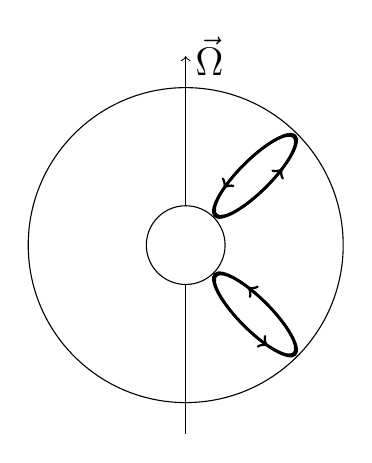
\begin{tikzpicture}
        \draw 
            (0,0) circle (2cm);
        \draw 
            (0,0) circle (0.5cm);
        \draw 
            (0,-2.4)--(0,-0.5);
        \draw
            [->, black] (0,0.5)--(0,2.4) node[anchor=west]{\Large $\vec{\Omega}$};
        \draw[rotate around = {-45:(0.88,0.88)},
        decoration={markings, mark=at position 0.625 with {\arrow{>}}},
        postaction={decorate}, line width = 1pt
        ]
            (0.88,0.88) ellipse (0.2 and 0.72);
        \draw[rotate around = {-45:(0.88,0.88)},
        decoration={markings, mark=at position 0.1 with {\arrow{>}}},
        postaction={decorate}, line width = 1pt
        ]
            (0.88,0.88) ellipse (0.2 and 0.7);
        \draw[rotate around = {45:(0.88,-0.88)},
        decoration={markings, mark=at position 0.625 with {\arrow{>}}},
        postaction={decorate}, line width = 1pt
        ]
            (0.88,-0.88) ellipse (0.2 and 0.72);
        \draw[rotate around = {45:(0.88,-0.88)},
        decoration={markings, mark=at position 0.1 with {\arrow{>}}},
        postaction={decorate}, line width = 1pt
        ]
            (0.88,-0.88) ellipse (0.2 and 0.7);
    \end{tikzpicture}
    \caption{Convective motion in a rotating stellar atmosphere.}
    \label{fig:rotatingconvection}
\end{figure}